\documentclass{article}

\usepackage{graphicx}
\usepackage{tikz}
\usepackage{tikzsymbols}
\usetikzlibrary{calc,patterns,shapes.geometric}
\pagestyle{empty}
\usepackage[margin=0pt]{geometry}
\geometry{papersize={14in,12in}}

\def\centerarc[#1](#2)(#3:#4:#5){\draw[#1] ($(#2)+({#5*cos(#3)},{#5*sin(#3)})$) arc (#3:#4:#5);}

\begin{document}
	\begin{figure}
		\centering
		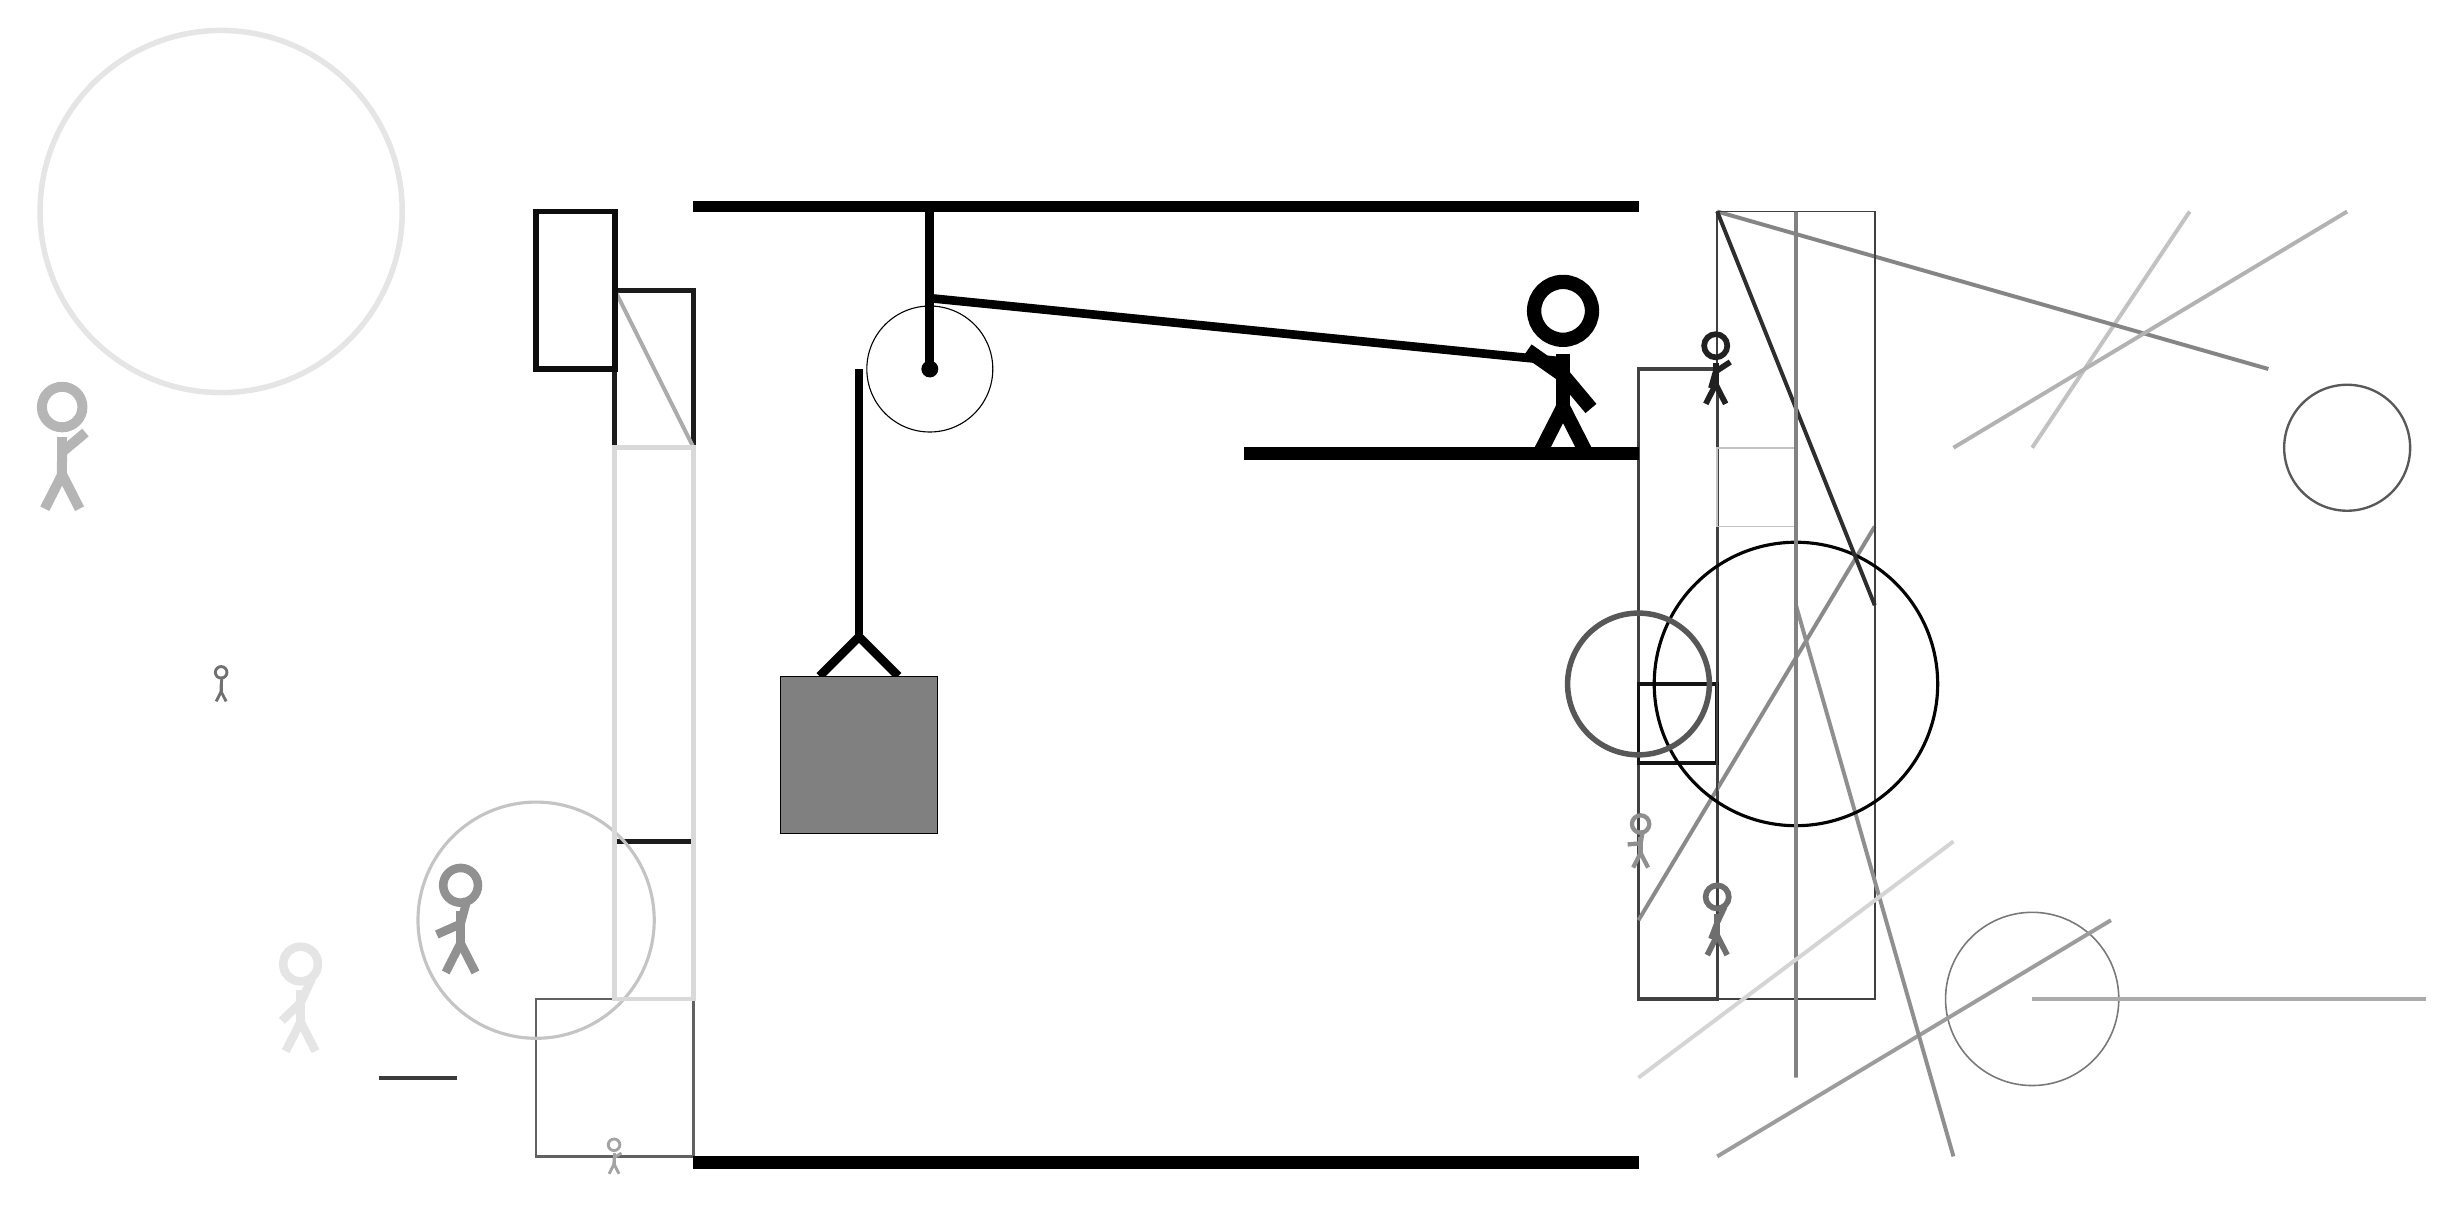
\begin{tikzpicture}
			%%%%% START %%%%%
			
			\draw[fill=black] (-2, 9) rectangle (10, 9.125);
			
			\draw (1, 7) circle (0.8);
			\draw[fill=black] (1, 7) circle (0.1);
			\draw[line width=1.1mm] (1, 9) -- (1, 7);
			
			\draw[line width=1.1mm](-0.4, 3.1) --  (0.1, 3.6) -- (0.6, 3.1);
			\draw[fill=black!50] (-0.9, 3.1) rectangle (1.1, 1.1);
			
			\draw[line width=0.5mm, color=black!24](15, 6) -- (17, 9);
			
			\draw[line width=0.4mm, color=black!74] (10, -1) rectangle (11, 7);
			\draw [line width=0.7mm, color=black!10](-8, 9) circle (2.3);
			\draw[line width=0.5mm, color=black!46](10, 0) -- (13, 5);
			\draw[line width=0.5mm, color=black!77](-5, -2) -- (-6, -2);
			\draw [line width=0.3mm, color=black!65](19, 6) circle (0.8);
			\draw [line width=0.2mm, color=black!53](15, -1) circle (1.1);
			\draw[line width=0.5mm, color=black!92] (10, 2) rectangle (11, 3);
			\draw[line width=0.5mm, color=black!48](11, 9) -- (18, 7);
			\draw[line width=0.2mm, color=black!75] (11, -1) rectangle (13, 9);
			
			\draw[line width=0.6mm, color=black!89] (-3, 1) rectangle (-2, 8);
			\draw[line width=0.5mm, color=black!33](-2, 6) -- (-3, 8);
			\draw[line width=0.3mm, color=black!62] (-2, -3) rectangle (-4, -1);
			
			\draw[line width=0.2mm, color=black!24] (11, 6) rectangle (12, 5);
			\node[line width=0.4mm, color=black!57] at (11, 0) {\Strichmaxerl[4][69][65]};
			\draw[line width=0.5mm, color=black!39](11, -3) -- (16, 0);
			
			\node[line width=0.4mm, color=black!36] at (-3, -3) {\Strichmaxerl[2][88][32]};
			\draw[line width=0.5mm, color=black!33](15, -1) -- (20, -1);
			\node[line width=0.7mm, color=black!44] at (10, 1) {\Strichmaxerl[3][5][80]};
			
			\draw [line width=0.4mm, color=black!23](-4, 0) circle (1.5);
			\draw[line width=0.5mm, color=black!44](14, -3) -- (12, 4);
			\draw[line width=0.6mm, color=black!15] (-3, -1) rectangle (-2, 6);
			\draw [line width=0.4mm, color=black!99](12, 3) circle (1.8);
			\draw[line width=0.5mm, color=black!30](14, 6) -- (19, 9);
			\node[line width=0.7mm, color=black!87] at (11, 7) {\Strichmaxerl[4][74][33]};
			\node[line width=0.7mm, color=black!56] at (-8, 3) {\Strichmaxerl[2][89][84]};
			
			\node[line width=0.4mm, color=black!29] at (-10, 6) {\Strichmaxerl[7][89][40]};
			\draw[line width=0.5mm, color=black!82](13, 4) -- (11, 9);
			\node[line width=0.7mm, color=black!43] at (-5, 0) {\Strichmaxerl[6][24][75]};
			
			\draw[line width=0.4mm, color=black!49] (12, 9) rectangle (12, -2);
			\draw[line width=0.7mm, color=black!95] (-3, 9) rectangle (-4, 7);
			
			\node[line width=0.5mm, color=black!10] at (-7, -1) {\Strichmaxerl[6][44][65]};
			\draw [line width=0.7mm, color=black!66](10, 3) circle (0.9);
			\draw[line width=0.5mm, color=black!17](14, 1) -- (10, -2);
			
			
			\draw[line width=1.1mm](0.1, 7) -- (0.1, 3.6);
			\centerarc[line width=1.1mm](1, 7)(90:180:0.9)
			\draw[line width=1.1mm](1, 7.9) -- (9, 7.1);
			
			\node at (9, 7) {\Strichmaxerl[10][-35][-50]};
			\draw[fill=black] (5, 6) rectangle (10, 5.85);
			
			\draw[fill=black] (-2, -3) rectangle (10, -3.15);
			
			%%%%% END %%%%%
		\end{tikzpicture}
	\end{figure}	
\end{document}